\documentclass[11pt, a4paper]{article}
\usepackage{pdfpages}
\usepackage{parallel}
\usepackage[T2A]{fontenc}
\usepackage{ucs}
\usepackage[utf8x]{inputenc}
\usepackage[polish,english,russian]{babel}
\usepackage{hyperref}
\usepackage{rotating}
\usepackage[inner=2cm,top=1.8cm,outer=2cm,bottom=2.3cm,nohead]{geometry}
\usepackage{listings}
\usepackage{graphicx}
\usepackage{wrapfig}
\usepackage{longtable}
\usepackage{indentfirst}
\usepackage{array}
\usepackage{tikzsymbols}
\usepackage{soul}
\usepackage[ruled,vlined]{algorithm2e}
%\counterwithout{figure}{section} 

\usepackage{url}
\makeatletter
\g@addto@macro{\UrlBreaks}{\UrlOrds}
\makeatother

\newcolumntype{P}[1]{>{\raggedright\arraybackslash}p{#1}}
\frenchspacing
\usepackage{fixltx2e} %text sub- and superscripts
\usepackage{icomma} % коскі ў матэматычным рэжыме
\PreloadUnicodePage{4}

\newcommand{\longpage}{\enlargethispage{\baselineskip}}
\newcommand{\shortpage}{\enlargethispage{-\baselineskip}}

\def\switchlang#1{\expandafter\csname switchlang#1\endcsname}
\def\switchlangbe{
\let\saverefname=\refname%
\def\refname{Літаратура}%
\def\figurename{Іл.}%
}
\def\switchlangen{
\let\saverefname=\refname%
\def\refname{References}%
\def\figurename{Fig.}%
}
\def\switchlangru{
\let\saverefname=\refname%
\let\savefigurename=\figurename%
\def\refname{Литература}%
\def\figurename{Рис.}%
}

\hyphenation{admi-ni-stra-tive}
\hyphenation{ex-pe-ri-ence}
\hyphenation{fle-xi-bi-li-ty}
\hyphenation{Py-thon}
\hyphenation{ma-the-ma-ti-cal}
\hyphenation{re-ported}
\hyphenation{imp-le-menta-tions}
\hyphenation{pro-vides}
\hyphenation{en-gi-neering}
\hyphenation{com-pa-ti-bi-li-ty}
\hyphenation{im-pos-sible}
\hyphenation{desk-top}
\hyphenation{elec-tro-nic}
\hyphenation{com-pa-ny}
\hyphenation{de-ve-lop-ment}
\hyphenation{de-ve-loping}
\hyphenation{de-ve-lop}
\hyphenation{da-ta-ba-se}
\hyphenation{plat-forms}
\hyphenation{or-ga-ni-za-tion}
\hyphenation{pro-gramming}
\hyphenation{in-stru-ments}
\hyphenation{Li-nux}
\hyphenation{sour-ce}
\hyphenation{en-vi-ron-ment}
\hyphenation{Te-le-pathy}
\hyphenation{Li-nux-ov-ka}
\hyphenation{Open-BSD}
\hyphenation{Free-BSD}
\hyphenation{men-ti-on-ed}
\hyphenation{app-li-ca-tion}

\def\progref!#1!{\texttt{#1}}
\renewcommand{\arraystretch}{2} %Іначай формулы ў матрыцы зліпаюцца з лініямі
\usepackage{array}

\def\interview #1 (#2), #3, #4, #5\par{

\section[#1, #3, #4]{#1 -- #3, #4}
\def\qname{LVEE}
\def\aname{#1}
\def\q ##1\par{{\noindent \bf \qname: ##1 }\par}
\def\a{{\noindent \bf \aname: } \def\qname{L}\def\aname{#2}}
}

\def\interview* #1 (#2), #3, #4, #5\par{

\section*{#1\\{\small\rm #3, #4. #5}}
\ifx\ParallelWhichBox\undefined%
    \addcontentsline{toc}{section}{#1, #3, #4}%
\else%
\ifnum\ParallelWhichBox=0%
    \addcontentsline{toc}{section}{#1, #3, #4}%
\fi\fi%

\def\qname{LVEE}
\def\aname{#1}
\def\q ##1\par{{\noindent \bf \qname: ##1 }\par}
\def\a{{\noindent \bf \aname: } \def\qname{L}\def\aname{#2}}
}

\newcommand{\interviewfooter}[1]{
\vskip 1em
\noindent \textit{#1}
}

\switchlang{en}
\begin{document}

\title{1992 "--- IBM ``Soap'' mouse}
\date{}
\maketitle
\selectlanguage{english}

This mouse, officially known by the hard-to-remember name ``model 13H6690'' (and almost identical ``model 33G5430'') was apparently released to the market in 1992 as an update to the 1987 IBM PS/2 mouse.
In addition to the obvious association with a well-rounded bar of soap, this model was also unofficially called ``IBM Fat Mouse''.

\begin{figure}[h]
    \centering
    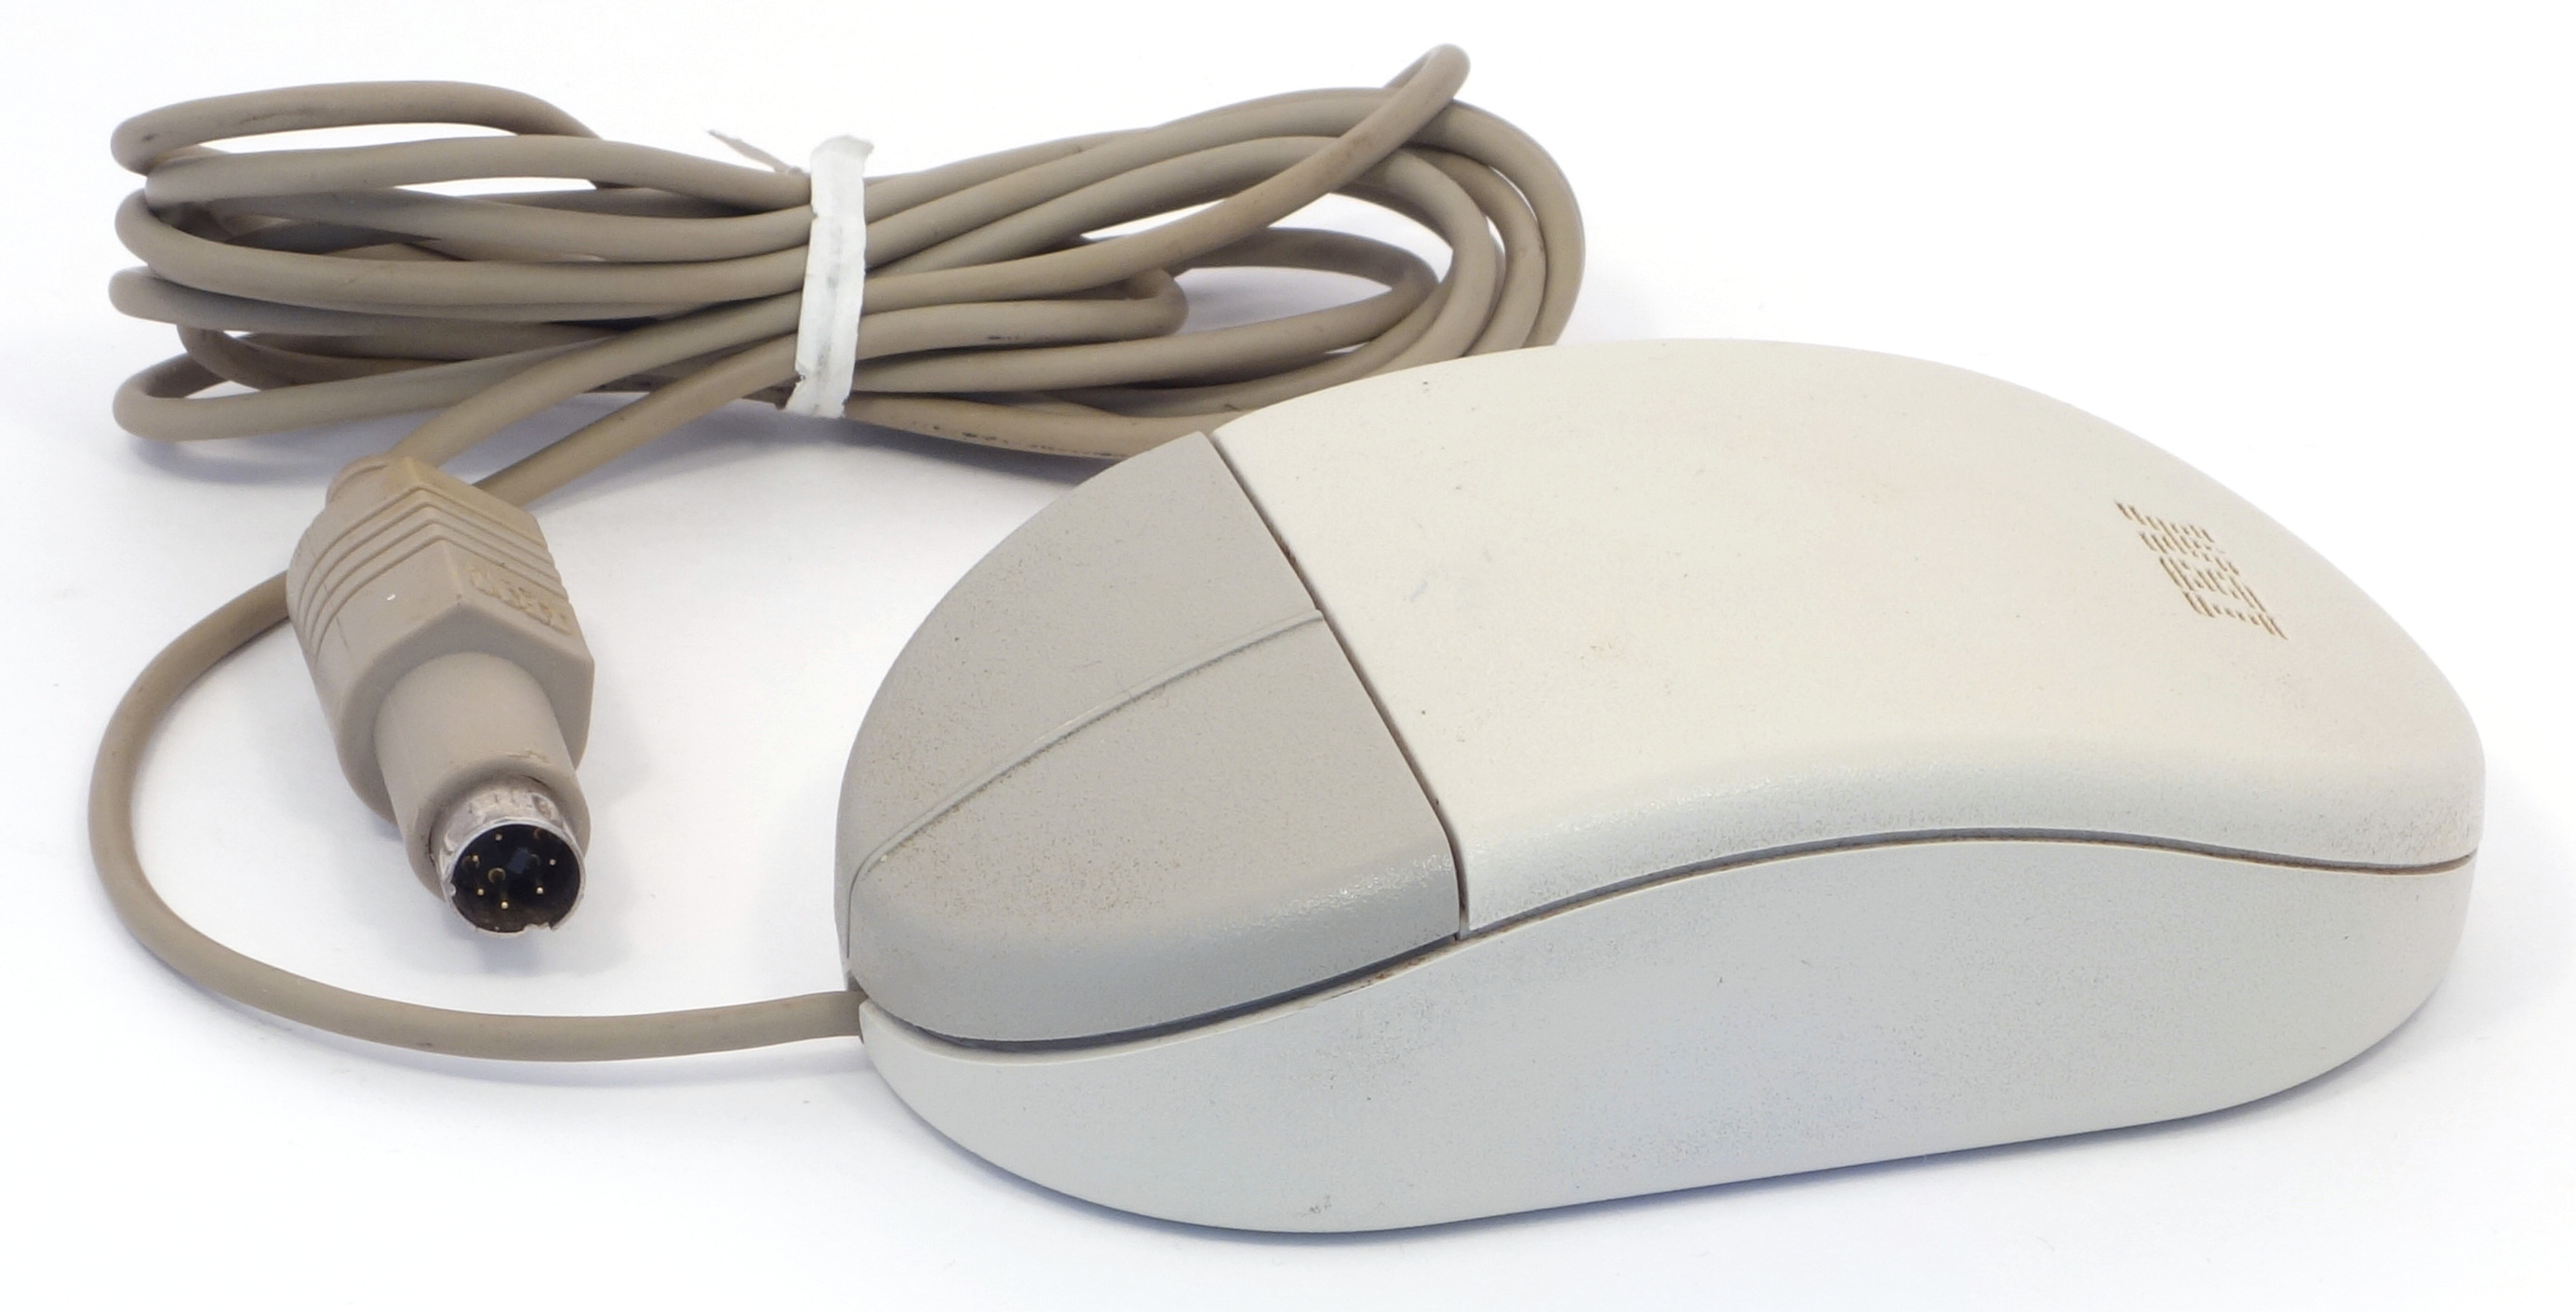
\includegraphics[scale=0.6]{1992_ibm_soap_mouse/pic_30.jpg}
    \caption{IBM Soap mouse}
    \label{fig:IBMSoapPic}
\end{figure}

Despite its wide distribution, this mouse is practically not represented in press reviews. IBM supplied it with some models of PS/1 and PS/ValuePoint computers (however, along with this mouse, you can find promotional materials for these computers with the previous IBM PS/2 Mouse model).

\begin{figure}[h]
    \centering
    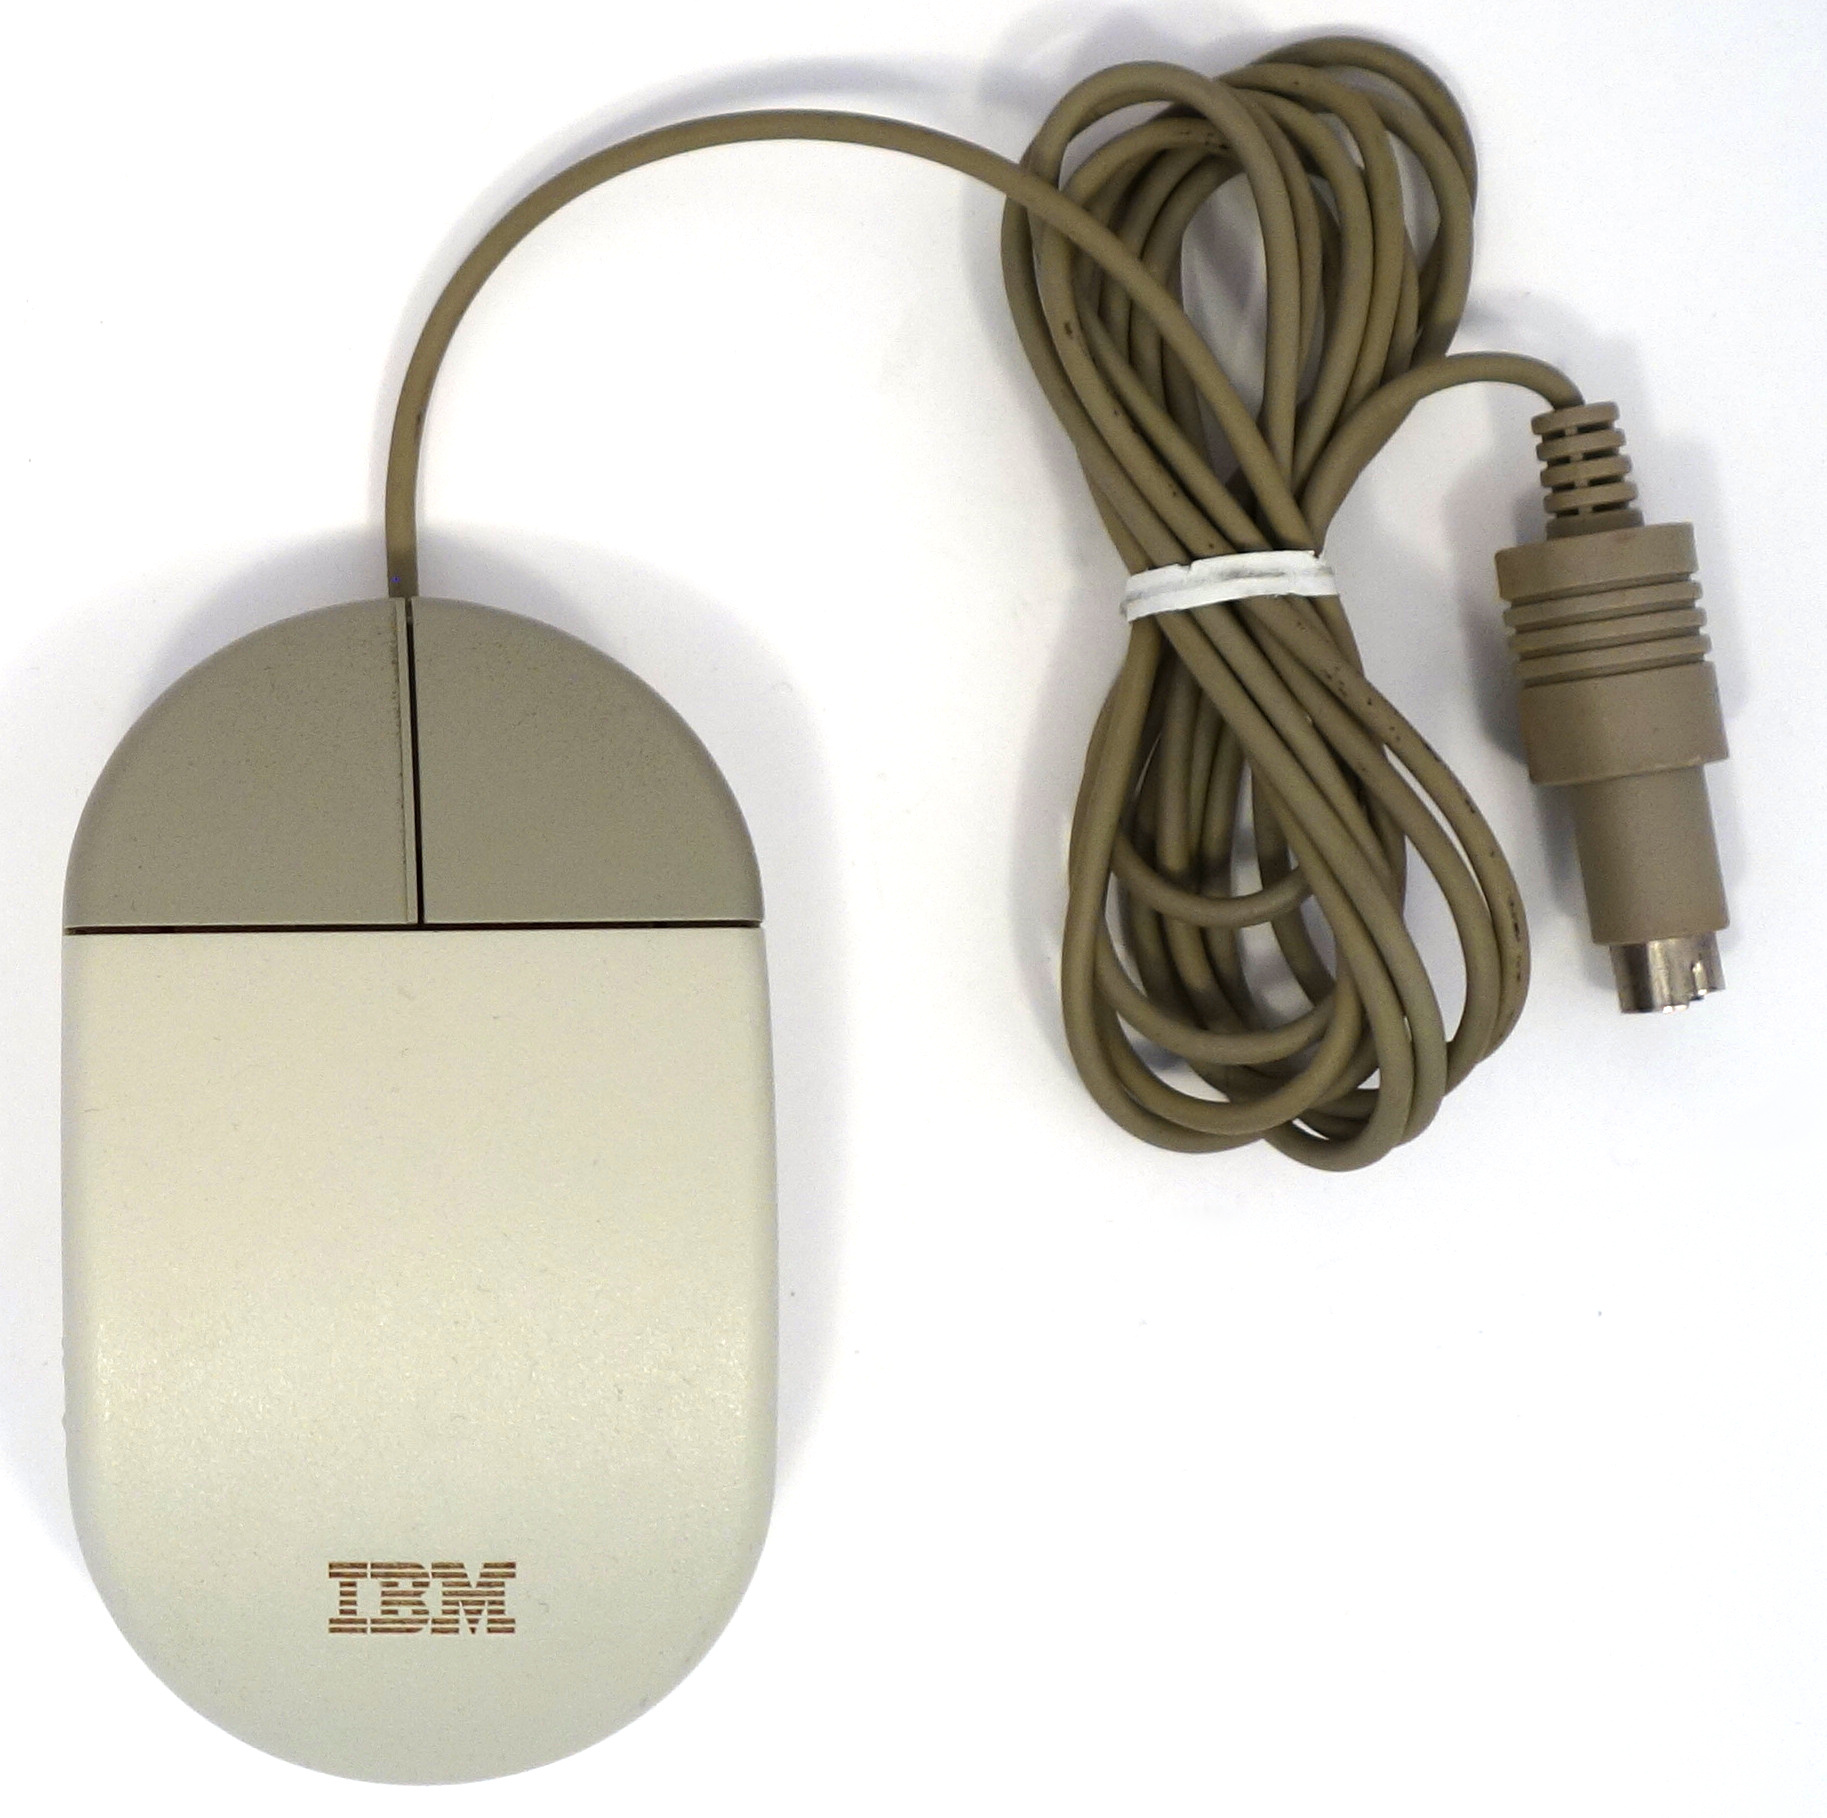
\includegraphics[scale=0.5]{1992_ibm_soap_mouse/top_60.jpg}
    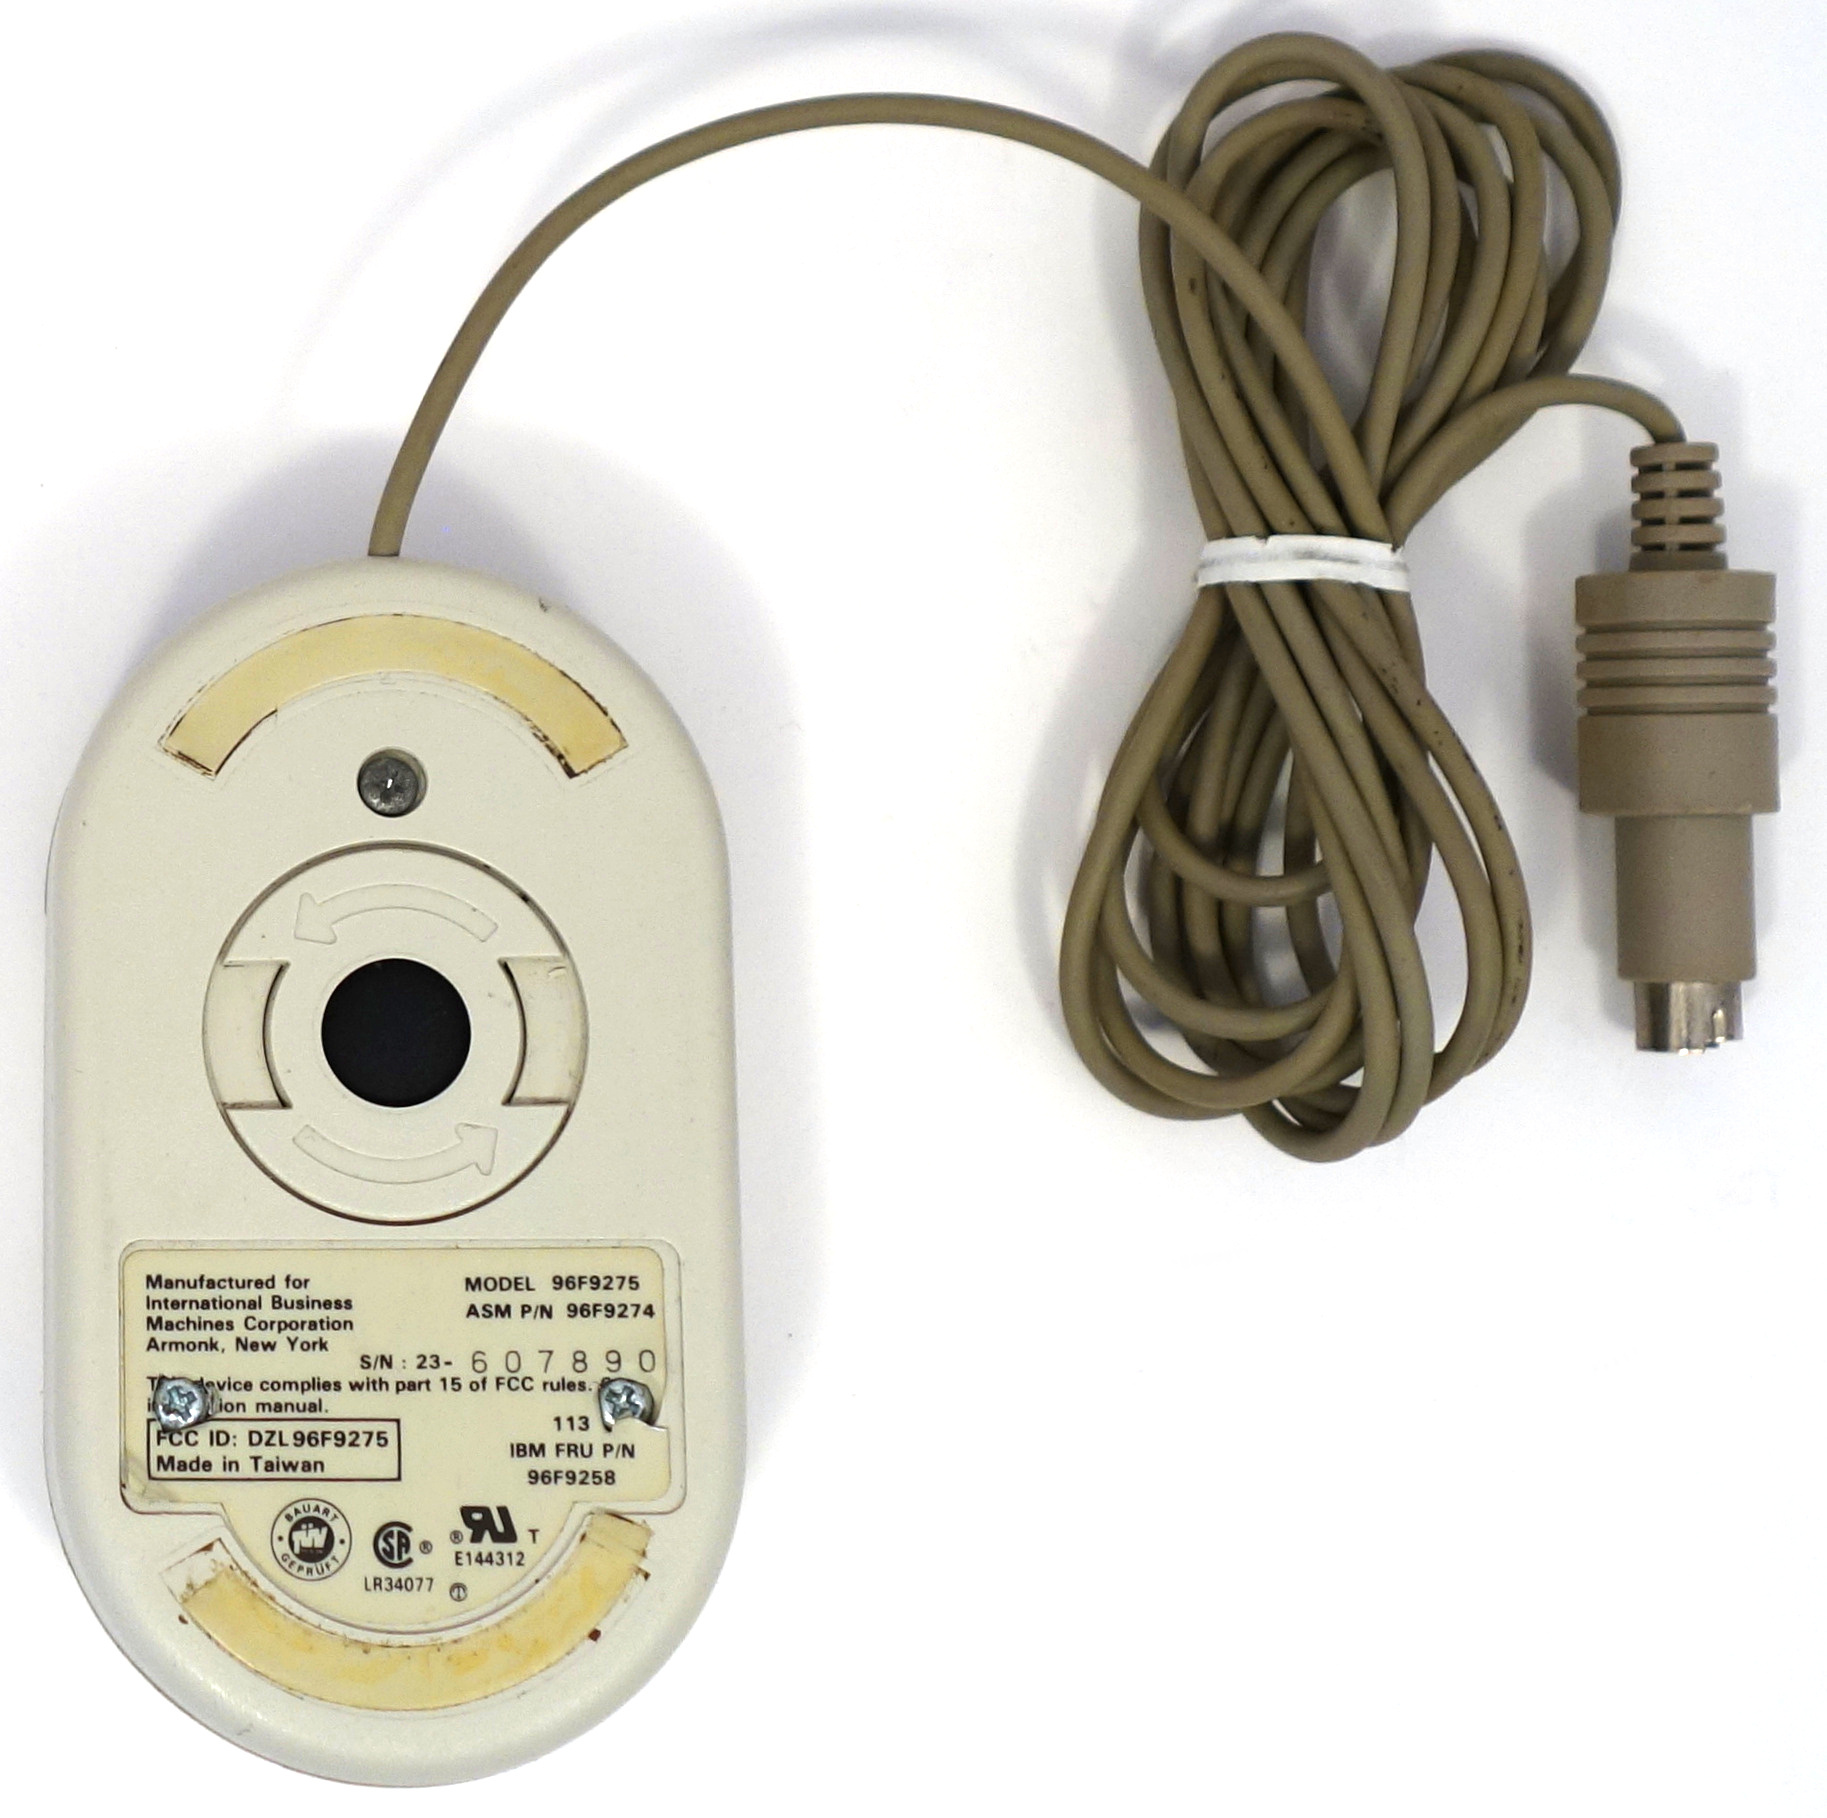
\includegraphics[scale=0.5]{1992_ibm_soap_mouse/bottom_60.jpg}
    \caption{IBM Soap mouse, top and bottom views}
    \label{fig:IBMSoapTopBottom}
\end{figure}

The mouse was produced in several color options: a solid beige body, and two-color versions with dark buttons (fig. \ref{fig:IBMSoapTopBottom}) or a dark lower part of the body \cite{hugold}. On the top side there are two large buttons and an engraved IBM logo; in general, the case is minimalistic and, apart from that, does not contain any additional elements. On the bottom you can see a ball and a swivel ring that allows you to remove it for cleaning.

\begin{figure}[h]
    \centering
    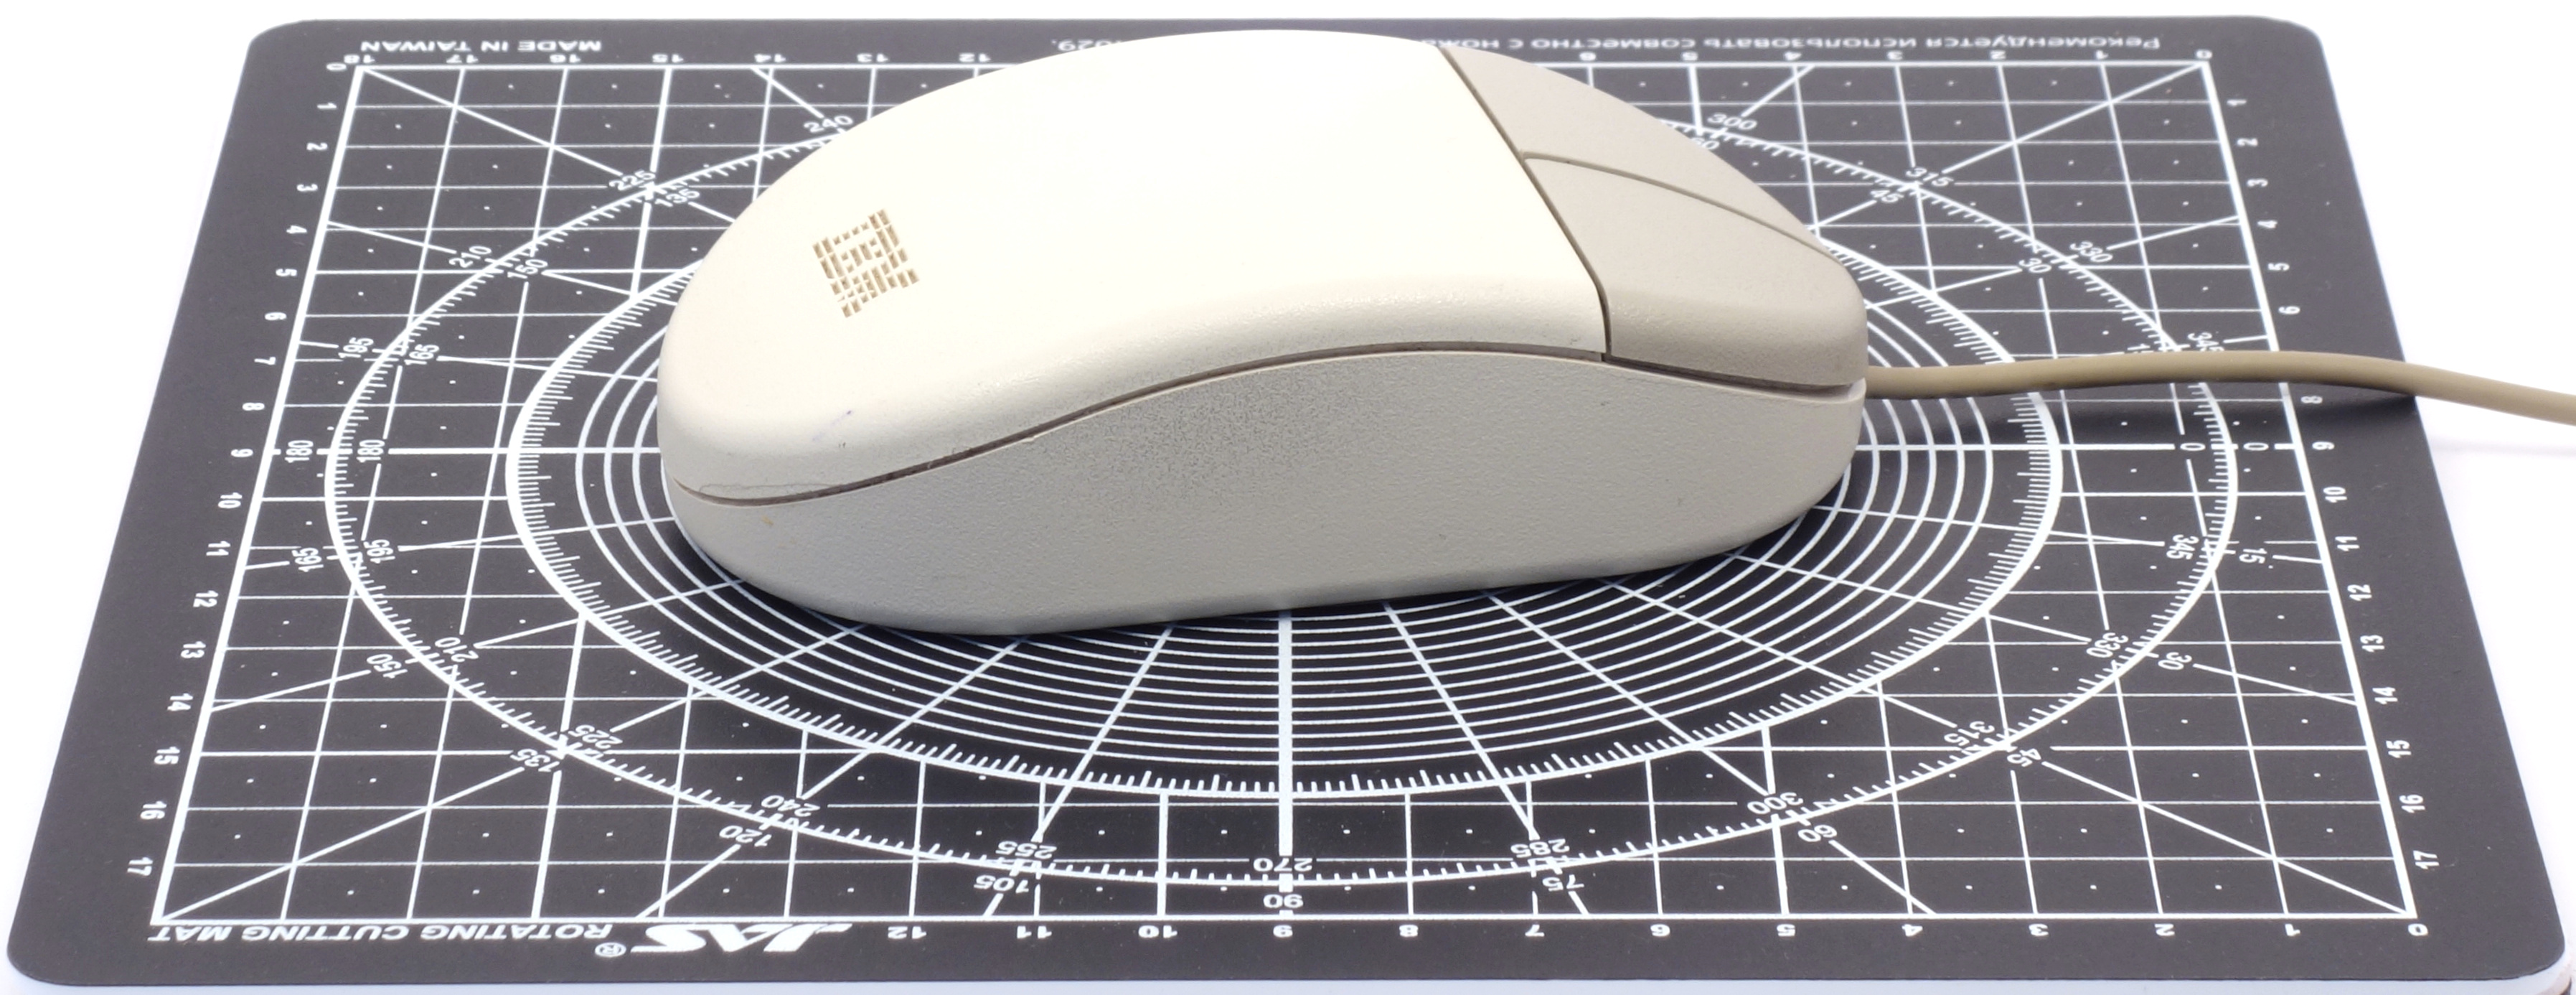
\includegraphics[scale=0.34]{1992_ibm_soap_mouse/size_30.jpg}
    \caption{IBM Soap mouse on a graduated pad with a grid step of 1~cm}
    \label{fig:IBMSoapSize}
\end{figure}

The mouse is compact in size (fig. \ref{fig:IBMSoapSize}) and does not provide wrist support. However, as can be seen in fig. \ref{fig:IBMSoapHand}, the curved shape of the body allows you to comfortably rest your palm on it and press the buttons in a natural hand position. At the same time, the mouse is symmetrical and is equally suitable for left-handers and right-handers. In addition to ergonomics, the mouse was also successful in terms of reliability \cite{usage}, which apparently made it popular and caused a fairly long mass production.

\begin{figure}[h]
    \centering
    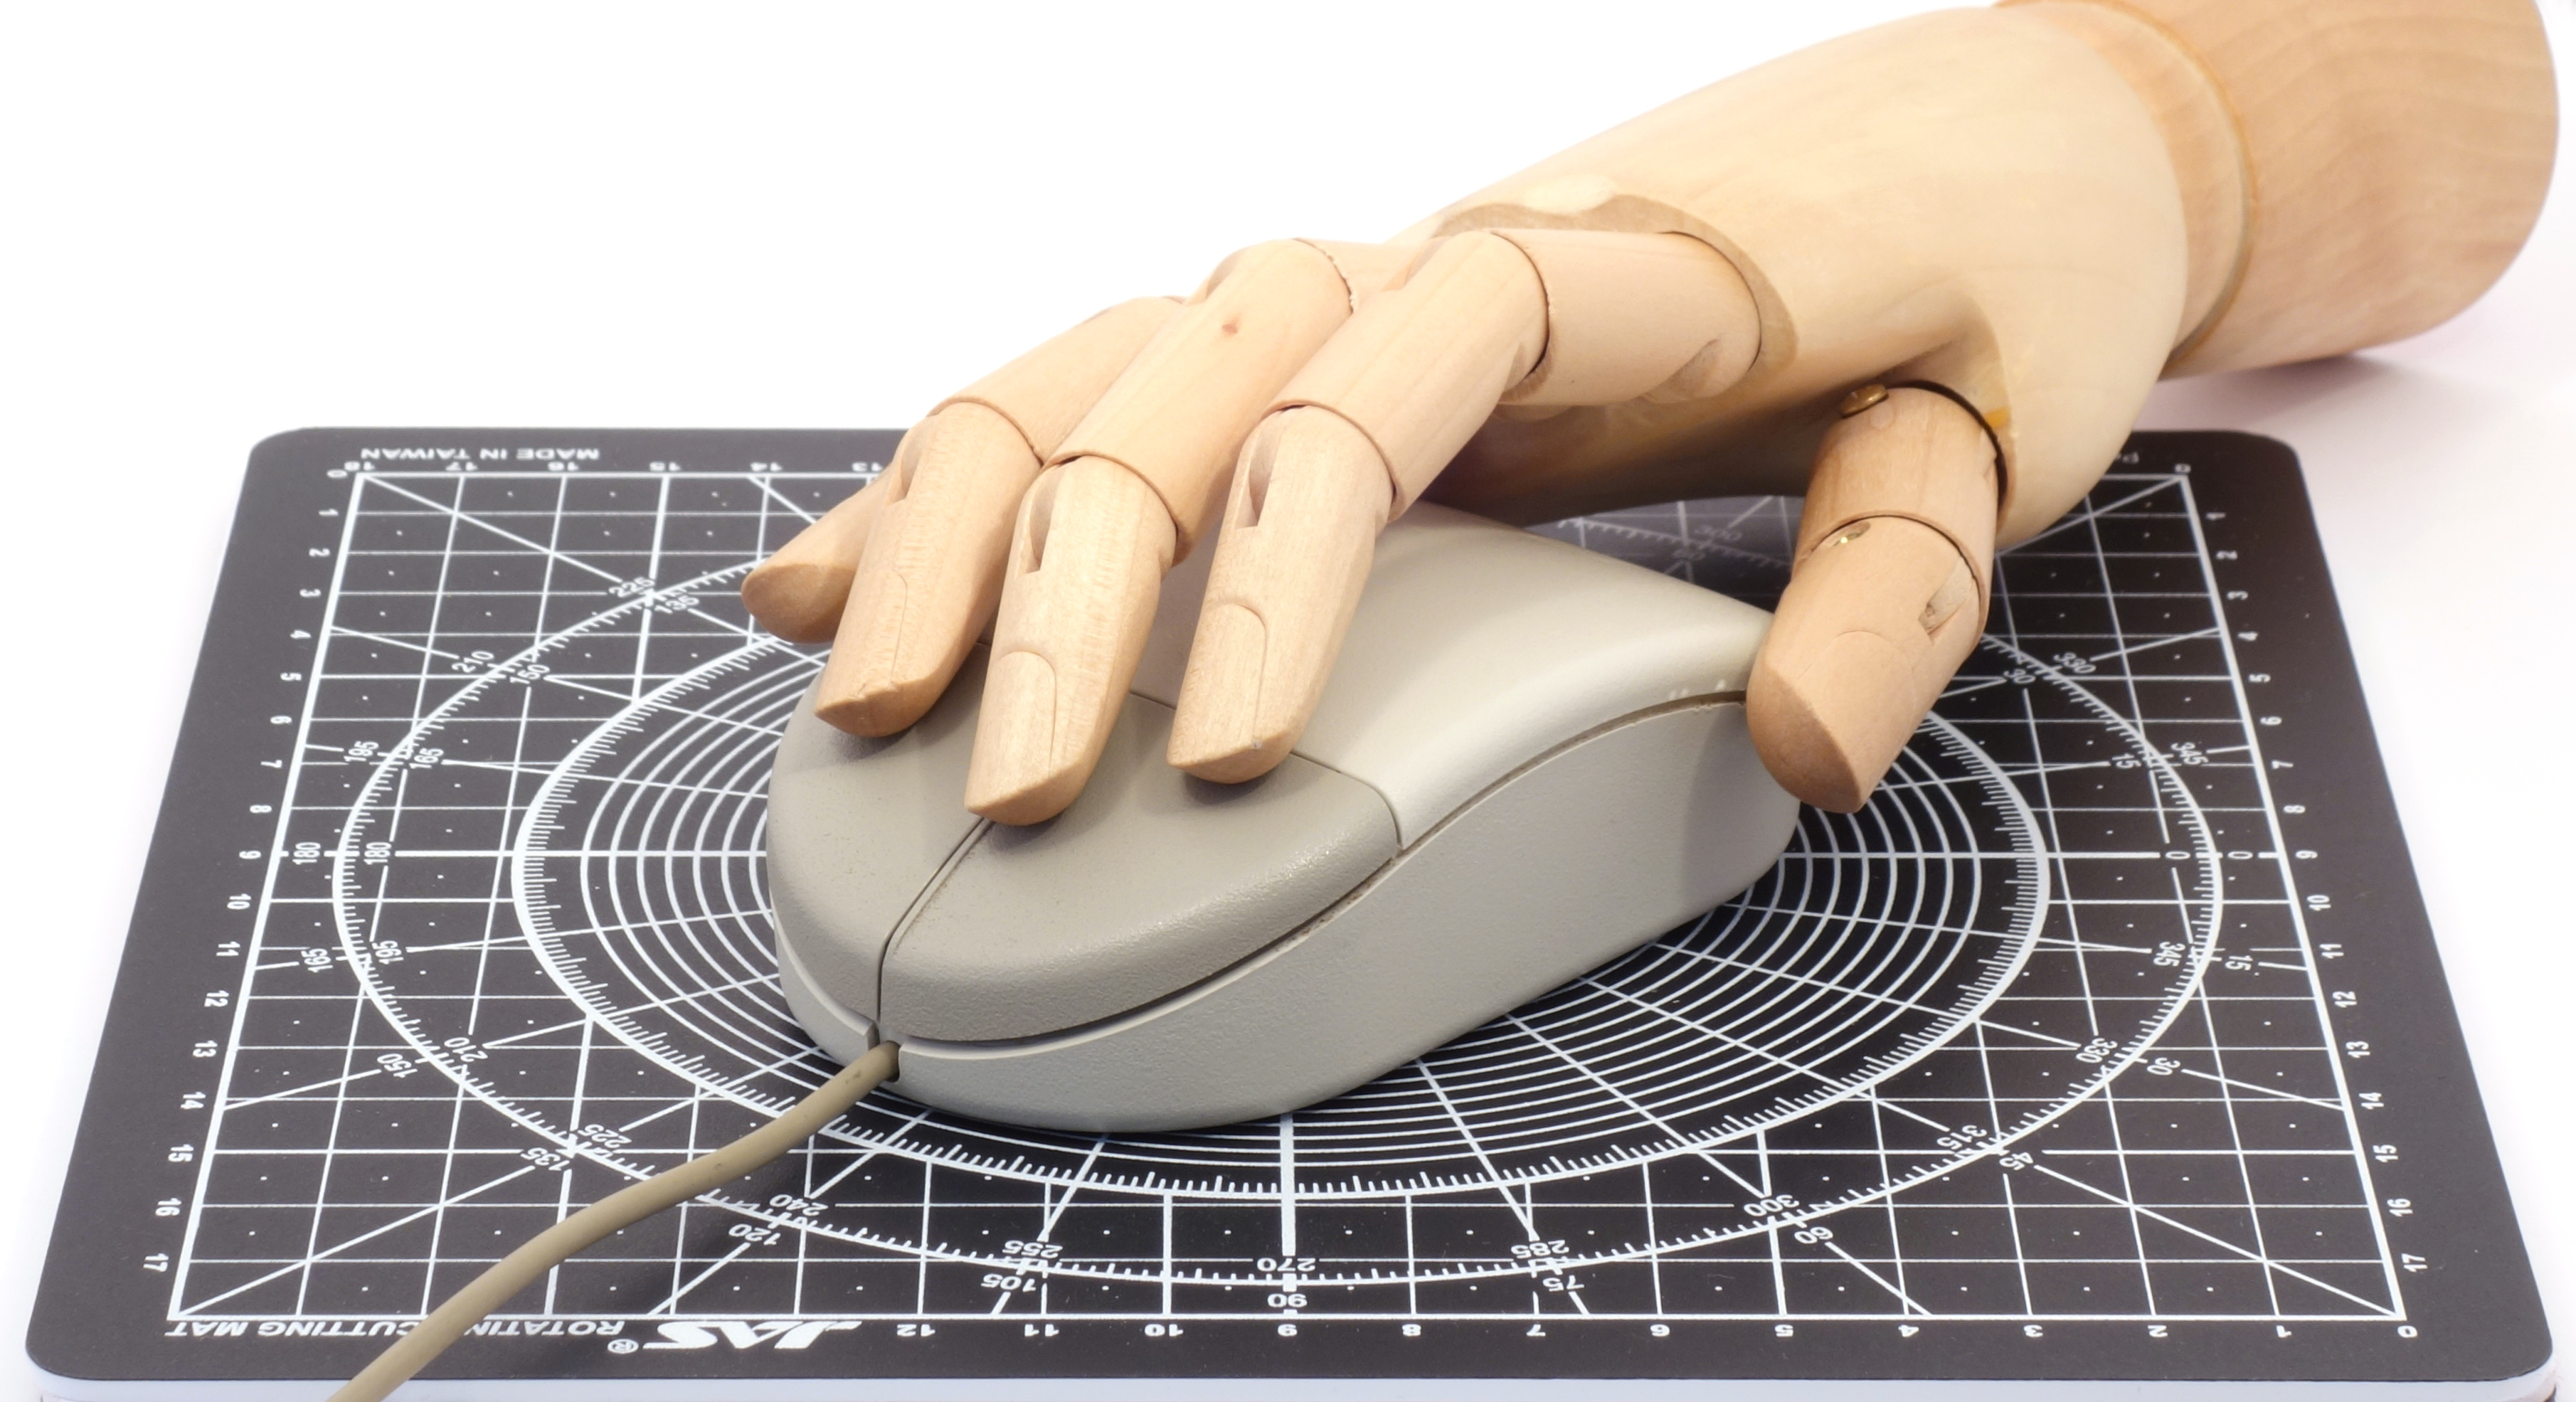
\includegraphics[scale=0.34]{1992_ibm_soap_mouse/hand_30.jpg}
    \caption{IBM Soap mouse with a human hand model}
    \label{fig:IBMSoapHand}
\end{figure}

The internals of the IBM Soap mouse are shown in fig. \ref{fig:IBMSoapInside}. This is an optomechanical encoder device manufactured by Logitech. The heavily slotted encoder disks, the low number of discrete PCB elements, and the plastic rollers are typical of mid-90s rather than early 90s mice, making the IBM Soap mouse one of the pioneers of this trend.

\begin{figure}[h]
    \centering
    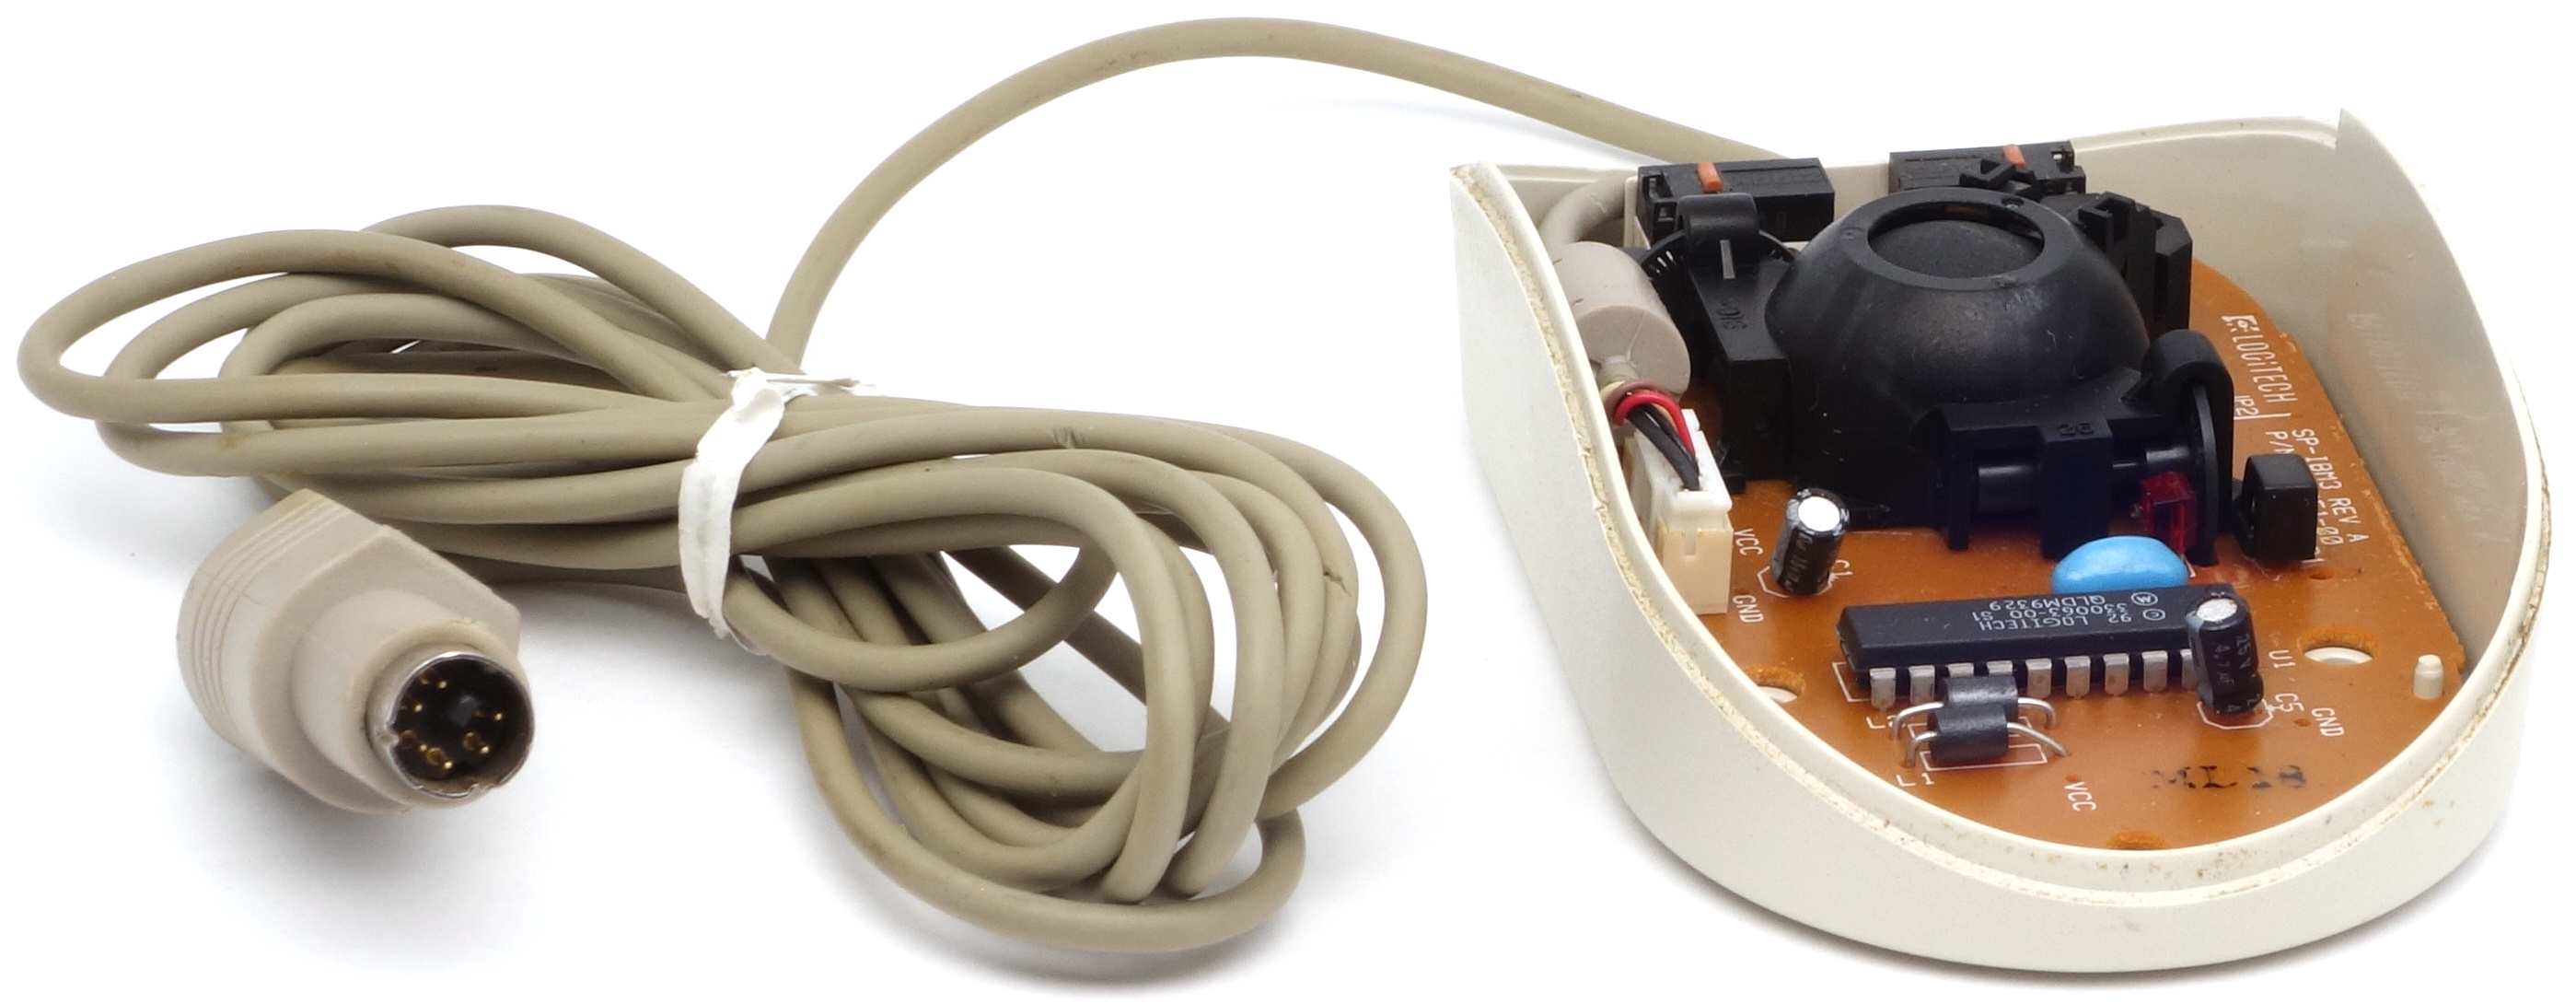
\includegraphics[scale=0.7]{1992_ibm_soap_mouse/inside_60.jpg} 
    \caption{IBM Soap mouse disassembled}
    \label{fig:IBMSoapInside}
\end{figure}

\begin{thebibliography}{9}
\bibitem {usage} Wendt P.H. Mice \& other stuff \url{http://www.mcamafia.de/mycomp/mycomp06.htm}
\bibitem {hugold} Przytul grata. IBM Mouse PS/2. \url{http://hugold.pl/gratym0126/ibm33g5430.html}
\end{thebibliography}
\end{document}
